\documentclass{standalone}
\usepackage{graphicx}	
\usepackage{amssymb, amsmath}
\usepackage{color}

\usepackage{tikz}
\usetikzlibrary{intersections, backgrounds}

\definecolor{light}{RGB}{220, 188, 188}
\definecolor{mid}{RGB}{185, 124, 124}
\definecolor{dark}{RGB}{143, 39, 39}
\definecolor{highlight}{RGB}{180, 31, 180}
\definecolor{gray10}{gray}{0.1}
\definecolor{gray20}{gray}{0.2}
\definecolor{gray30}{gray}{0.3}
\definecolor{gray40}{gray}{0.4}
\definecolor{gray60}{gray}{0.6}
\definecolor{gray70}{gray}{0.7}
\definecolor{gray80}{gray}{0.8}
\definecolor{gray90}{gray}{0.9}
\definecolor{gray95}{gray}{0.95}

\newcommand*{\offset}{0.025}

\begin{document}

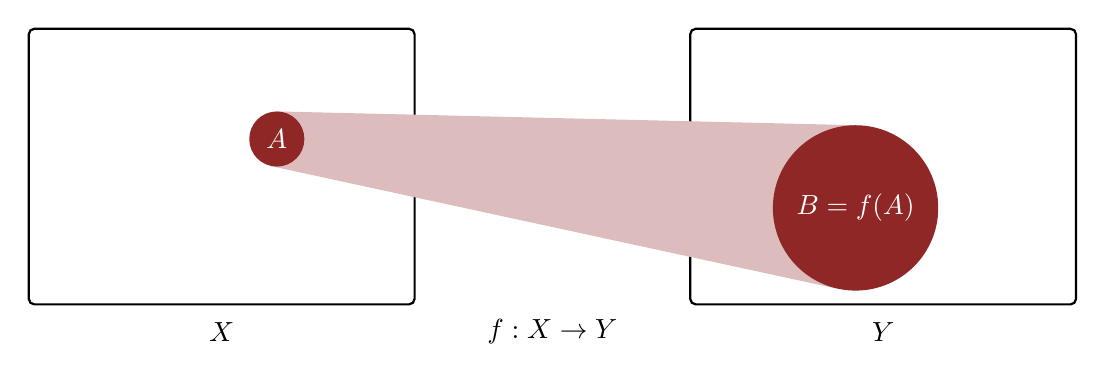
\begin{tikzpicture}[scale=0.35, thick]
  \draw [rounded corners=2pt, color=black] (-5, 0) rectangle +(-14, 10);
  \node[] at (-12, -1) { $X$ };

  \draw [rounded corners=2pt, color=black] (5, 0) rectangle +(14, 10);
  \node[] at (12, -1) { $Y$ };
  
  \node at (0, -1) { $f: X \rightarrow Y$ };
  
  \fill [color=light] (-10, 7.002) -- (11, 6.501) -- (10.3, 0.576) -- (-10.2, 5.015) -- cycle;
  
  \fill [fill=dark, text=white] (11, 3.5) circle (3)
  node { $B = f(A)$ };
  
  \fill [fill=dark, text=white] (-10, 6) circle (1)
  node { $A$ };
    
\end{tikzpicture}

\end{document}  